%% 
%% Copyright 2019-2020 Elsevier Ltd
%% 
%% This file is part of the 'CAS Bundle'.
%% --------------------------------------
%% 
%% It may be distributed under the conditions of the LaTeX Project Public
%% License, either version 1.2 of this license or (at your option) any
%% later version.  The latest version of this license is in
%%    http://www.latex-project.org/lppl.txt
%% and version 1.2 or later is part of all distributions of LaTeX
%% version 1999/12/01 or later.
%% 
%% The list of all files belonging to the 'CAS Bundle' is
%% given in the file `manifest.txt'.
%% 
%% Template article for cas-dc documentclass for 
%% double column output.

%\documentclass[a4paper,fleqn,longmktitle]{cas-dc}
\documentclass[a4paper,fleqn]{cas-dc}

%\usepackage[authoryear,longnamesfirst]{natbib}
%\usepackage[authoryear]{natbib}
\usepackage[numbers]{natbib}
\usepackage{amsmath,booktabs}
\usepackage{lineno}
\modulolinenumbers[5]
\usepackage{graphicx} 
\usepackage[font=small,labelfont=bf]{caption}
\usepackage{subcaption}

\usepackage{algorithm}% <=================http://ctan.org/pkg/algorithms
\usepackage{algpseudocode}% <========== http://ctan.org/pkg/algorithmicx
\usepackage{hyperref} % <===============================================
\newcommand\vn[1]{\textsc{\MakeLowercase{#1}}} % "variable name" macro
\newcommand\mc[1]{\multicolumn{1}{c}{#1}} % handy shortcut macro
\newcommand\ID{\mathit{ID}}
\makeatletter
\newcommand*{\rom}[1]{\expandafter\@slowromancap\romannumeral #1@}
\makeatother

%%%Author definitions
\def\tsc#1{\csdef{#1}{\textsc{\lowercase{#1}}\xspace}}
\tsc{WGM}
\tsc{QE}
\tsc{EP}
\tsc{PMS}
\tsc{BEC}
\tsc{DE}
%%%

\begin{document}
\let\WriteBookmarks\relax
\def\floatpagepagefraction{1}
\def\textpagefraction{.001}
\shorttitle{A New Key Establishment Protocol}
\shortauthors{Sedat Akleylek et~al.}

\title [mode = title]{A New Key Establishment Protocol Based-on SIS Problem}          
\tnotemark[1,2]

\tnotetext[1]{This document is the results of the research
   project funded by the TUBITAK under grant no. EEEAG-116E279.}


\author[1]{Sedat Akleylek}[orcid=0000-0000-0000-0000]     
\cormark[1]
\ead{sedat.akleylek@bil.omu.edu.tr}

\author[1]{Nursah \c{C}evik}
\fnmark[1]
\ead{nursah.kaya@bil.omu.edu.tr}

\address[1]{Department of Computer Engineering, Faculty of Engineering, Ondokuz Mayis University, Samsun, Turkey}




\cortext[cor1]{Corresponding author}
%\cortext[cor2]{Principal corresponding author}
\fntext[fn1]{Nurşah \c{C}evik is partially funded by YÖK 100/2000 scholarship}




\begin{abstract}
	As a result of the increasing computing power with the quantum computing notion, it is predicted that the cryptosystems used today will not be reliable. Therefore, studies on cryptosystems that are reliable after quantum increased. The lattice-based systems become prominent in post-quantum cryptosystem design with their high-security level and small key sizes. The Short Integer Solution (SIS) problem proposed by Ajtai is known to be one of the difficult problems defined on lattice structures. Although several key exchange protocols based on the SIS problem have been proposed up to this time, these protocols have proven to be insecure against attacks. In this study, we present the CCA2 secure key encapsulation mechanism using the GUPTA encryption system based on the SIS and the non-homogeneous Short Integer Solution (ISIS) problems, presented in 2017. We then propose a new lattice-based key establishment protocol using the key encapsulation mechanism. Finally, we present a sample parameter set and a security analysis of the proposed protocol.
	
\end{abstract}

\begin{graphicalabstract}
	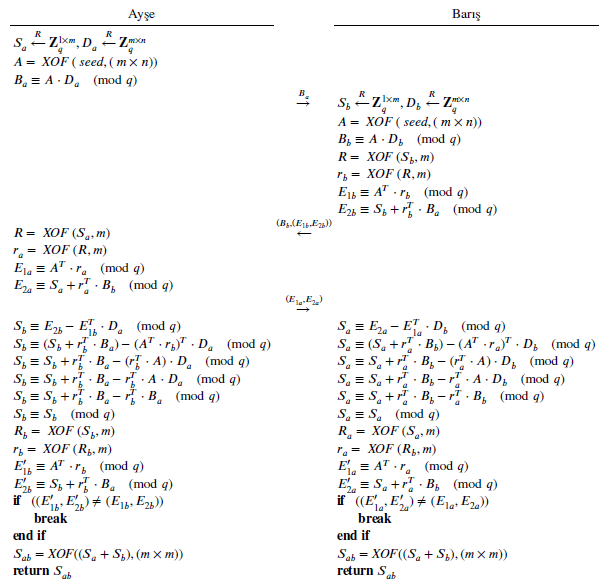
\includegraphics{figs/graphical_abstract.png}
\end{graphicalabstract}

\begin{highlights}
	\item Highlights
\end{highlights}

\begin{keywords}
	Key establishment protocol \sep Key encapsulation mechanishm \sep Post-quantum \sep Lattice-based \sep CCA2 \sep SIS
\end{keywords}


\maketitle



\section{Introduction}

	Several problems related to the security of cryptosystems were encountered with the introduction of the concept of quantum computing into our lives. The difficulties of many cryptosystems, whose reliability is accepted by various institutions such as NIST, ISO, IETF, and BSI, are based on discrete logarithm and factorization problems. The cryptosystems based on these problems have proved to be unreliable by Shor's Algorithm [1]. These cryptosystems are used in many applications used today. For example, in some security protocols such as SSL [2] and SSH [3], which enable us to establish secure communication on the internet, DH [4] and ECDH [5] systems or RSA [6] public-key encryption system are used as key establishment protocols. It is known that many public-key systems such as RSA, DSA, DH, ECDH are not reliable post-quantum. Studies on quantum-resistant cryptosystems are important as we need new systems that are secure against post-quantum attacks. In the literature, there are five different classes of cryptosystems, which are thought to be reliable against quantum attacks, such as cage-based, isogenic-based, code-based, and mixed-based cryptosystems. In 2004, Regev [11] introduced a new cryptographic structure based on the u-SVP problem and provided an alternative to Ajtai's system. In a study published in 2005, it showed the reliability of the LWE problem in truss structures [12]. Many cryptosystems have been identified on the lattice-based problems presented in the literature. In recent years, lattice-based cryptosystems attracted attention due to their worst case provable security levels, small size key structures, and processing speeds. Therefore, the interest in lattice-based cryptosystems increased considerably, and studies in this area gained value. 

	American National Institute of Standards and Technology (NIST) announced the need for reliable public-key cryptosystems after quantum in 2016 [15] and launched a competition in 2017 that looked for reliable system classes that can be used as a standard after quantum [16]. In the first round of the contest, the 69 cryptosystems, the 47 of which are public-key encryption and the 22 key digital signatures, were presented. The 17 candidates accepted to the second round of the competition. The 8 of second-round candidates are lattice-based cryptosystems: LAC, NewHope, NTRU, NTRU Prime, FrodoKEM, CRYSTALS-KYBER, SABER, and Round5. It is observed that the number of lattice-based systems is high among the presented systems. In general, cryptographic systems are used in three different application fields: encryption, digital signature, and key establishment. Key establishment is one of the application areas where security protocols are required after quantum computers. Key establishment protocols such as discrete logarithm-based DH are known to be not reliable against quantum computer attacks. Therefore, there is a need for quantum-resistant key establishment protocols.

	Another approach to key establishment protocols is the key encapsulation mechanism (KEM). This idea was first presented by Fujisaki and Okamoto [18]. Using KEM, Fujisaki and Okamoto have demonstrated how to transform a public key encryption system that is weak against adaptive chosen ciphertext attack (CCA2), into a cryptographically strong key establishment protocol. For this reason, in recent studies, while an OW-CCA2 secure key establishment protocol is designed, the use of KEM is preferred instead of the complex padding mechanism. For example, FrodoKEM, Crystals-Kyber, and NTRU-HRSS-KEM protocols [17].

\subsection{Motivation and Contribution}

	It is known that the SIS problem is one of the significant problems proven to be secure on lattice structures by Ajtai [7]. Various key establishment protocols based on the SIS problem are suggested. However, these protocols are proven to be insecure against attacks. It is known that it is very difficult to design a key exchange problem based only on the SIS problem [24].  In 2017, GUPTA  et.al. suggested a cryptosystem based on the SIS problem using the padding mechanism of the El-Gamal [13] system. Then, they proposed an encryption protocol and digital signature protocol [14]. The GUPTA cryptosystem is an efficient system as its computational complexity depends only on addition and multiplication between matrices and vectors [14]. Therefore, in this paper, we propose a secure key encapsulation mechanism of OW-CCA2 based on the OW-CPA secure GUPTA cryptosystem. After that, we suggest a new lattice-based key establishment protocol using the proposed KEM. Finally, we give a detailed security analysis.
\subsection{Organization}

	The manuscript was organized as follows. In Chapter 2, we gave definitions and representations about systems for a better understanding of the cryptosystems. In Chapter 3, we explained the GUPTA encryption protocol, and then proposed OW-CPA secure key generation, encryption and decryption algorithms for the protocol. At the beginning of Chapter 4, we proposed an OW-CCA2 secure KEM using the OW-CPA secure encryption protocol afterward suggested an OW-CCA2 secure key establishment protocol using the proposed KEM and gave a detailed security analysis. The results of this manuscript are summarized in Chapter 5.

\section{PRELIMINARIES}

	In this section, principal definitions and demonstrations about the proposed system are given.

\subsection{Notations}


\subsection{SIS and ISIS Problems}





\subsection{Semantic Security}

	The notation of semantic security implies that an attacker would have no knowledge of plaintext using the ciphertext obtained. These kinds of attacks are called passive attacks. However, in practice, systems are also required to be secure against active attacks. For this reason, different security notions such as CPA, CCA, CCA2 emerged. These notions are described in detail in Section 4.5.3. 
	
	In order to establish a secure key establishment protocol against CCA and CCA2 attacks, some operations must be added to the encryption system. The most significant one of these operations is hash functions which are the structure that provides the cryptographic randomness of the system.

\subsection{Extendable Output Function/XOF}


\section{OW-CPA SECURE GUPTA PUBLIC KEY CRYPTOSYSTEM}
	In this section, we define the parameters of the OW-CPA secure GUPTA public key cryptosystem and explain the system in detail. Then, we recommend the key generation, encryption, and decryption algorithms for OW-CPA secure GUPTA public key encryption system. A cryptosystem consists of three principal steps: key generation, encryption, and decryption. In Figure 1, the steps and parameter selection of the OW-CPA secure GUPTA cryptosystem are shown.

	\begin{figure}
		\centering
			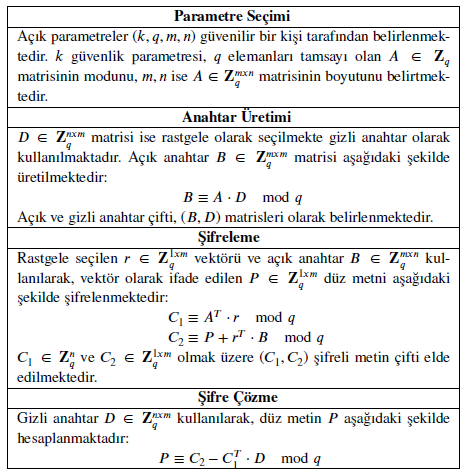
\includegraphics[scale=.7]{figs/fig1.png}
		\caption{OW-CPA Secure GUPTA Public Key Cryptosystem}
		\label{FIG:1}
	\end{figure}









\subsection{Key Generation}

	In this section, we describe the key generation algorithm we recommend for the OW-CPA secure GUPTA public key encryption system. In the KEY$\_$GENERATION algorithm given in Algorithm \ref{Algorithm:1}, the production steps of secret and public keys are given in detail.

	\begin{algorithm}
		\captionof{algorithm}{Key Generation}\label{keygen}
		\begin{algorithmic}
			\Procedure{KEY$\_$GENERATION }{$ seed $}
			\State $ D \overset{R}{\longleftarrow}  \mathbf{Z}_q^{m \times n} $ 
			\State $ A = \textit{ XOF } (\textit{ seed}, (\textit{ m $\times$ n}))$ 
			\State $ B   \equiv A \cdot D \pmod q $
			\State \Return $ (D, A, B) $ \Comment{Secret and Public keys}
			\EndProcedure
		\end{algorithmic}
		\label{Algorithm:1}
	\end{algorithm}

	The $ KEY\_GENERATION $ algorithm takes the $ seed $ variable explicitly shared by a trusted institution as the input value and starts the process by randomly selecting the secret key $ D $ matrix from the space of $Z_q^{n \times m}$. Then the algorithm calls $ XOF $ using the input values of $ seed $ and $ n \times m $ and gives the public parameter $ A $ matrix as output. Then $B \equiv A \cdot D mod q$ operation is calculated to obtain the public key B matrix. The secret key $ D $ matrix are produced by multiplying the public key $ B $ and the public parameter $ A $, and the algorithm terminates.




\subsection{OW-CPA Secure Encryption}

	In this section, we recommend for encryption and decryption algorithms for the OW-CPA secure cryptosystem. Then we explain the steps of the algorithms in detail. Encryption and decryption algorithms of the GUPTA cryptosystem are given in Figure 3.

	\begin{algorithm}
			\captionof{algorithm}{ENCRYPTION}
			\begin{algorithmic}
				\Procedure{ENCRYPTION}{$P$, $R$, $ A $, $ B $}
				\State $ r = \textit{ XOF } (\textit{ R}, \textit{ m}) $
				\State $ C_1 \equiv A^T \cdot r \pmod q $
				\State $ C_2 \equiv P + r^T \cdot B \pmod q $ 
				\State \Return $ (C_1, C_2) $ \Comment{Ciphertexts}
				\EndProcedure 
			\end{algorithmic}
		\label{Algorithm:2}
	\end{algorithm}

	The first step of public-key encryption is encryption. At the beginning of the encryption phase, the $ ENCRYPTION $ algorithm takes plain text $ P $, random value $ R $ vectors, and public parameter $ A $, public key $ B $ matrices as input. After that, $ XOF $ gives the random vector $ R $ as output by taking the random value $ R $ and length $ m $ as input. Then the algorithm multiplies the random vector $ r $ and the transpose of the public parameter $ A $ matrix in modulo $ q $ and computes the $ C_1 $ ciphertext. Consequently, it multiplies the matrix $ B $ and the transpose of the random vector $ r  $ and adds it to the plaintext vector $ P $ in modulo $ q $. In this step, the plaintext $ P $ is hidden by using the El-Gamal padding mechanism and generates the second ciphertext vector $ C_2 $. As a result of the encryption phase, it produces the ciphertext pair $ C_1 $ and $ C_2 $.

	\begin{algorithm}
		\captionof{algorithm}{DECRYPTION}\label{decrypt}
		\begin{algorithmic}
			\Procedure{DECRYPTION}{$C_1$, $ C_2 $, $ D $}
			\State $ P   \equiv C_2 - C_1^T \cdot D \pmod q$
			\State \Return $ P $ \Comment{Plaintext}
			\EndProcedure 
		\end{algorithmic}
		\label{Algorithm:3}
	\end{algorithm}

	The second step of public-key encryption is decryption. The $ DECRYPTION $ algorithm runs to decrypt the ciphertext pair $ C_1, C_2 $ vectors. The algorithm, which takes the secret key $ D $ matrix and the ciphertext pair $ C_1, C_2 $ vectors as input, calculates the $ P \equiv C_2 - C_1^T \cdot D mod q $ equation and returns the plaintext $ P $ vector.
	
	\textbf{Proof of Correctness}: We show that the parties in the OW-CPA secure GUPTA cryptosystem can obtain the plaintext from the encrypted text using the secret key.


	\begin{eqnarray}
		\textbf{P}^1 &=& \textbf{C}_2 - \textbf{C}_1^T\cdot \textbf{D} mod \quad q \nonumber \\
		&=& \textbf{P} + \textbf{r}^T\cdot \textbf{B} - (\textbf{r}^T \cdot \textbf{A})\cdot \textbf{D}\quad mod \quad q \nonumber \\
		&=& \textbf{P} + \textbf{r}^T\cdot \textbf{B} - \textbf{r}^T \cdot \textbf{A}\cdot \textbf{D}\quad mod \quad q	\nonumber \\
		&=& \textbf{P} + \textbf{r}^T\cdot \textbf{B} - \textbf{r}^T \cdot \textbf{B} \quad [\textbf{B} = \textbf{A}\cdot \textbf{D}]\quad mod \quad q \nonumber  \\
		&=& \textbf{P}\quad mod \quad q \nonumber
	\end{eqnarray}

\subsection{Complexity Analysis}
In this section, we provide a detailed performance analysis for the key generation, encryption, and decryption steps of the OW-CPA secure GUPTA cryptosystem. The performance of cryptosystems depends on the size of the parameters used. The parameter dimensions are taken as $ q = k^2, m = 2k \cdot log k $ and $ n = 4k \cdot log k $ ( $ k $ is security parameter). From here, $ | q | = log q $ equation is obtained. The complexities of the key generation, encryption, and decryption steps of the GUPTA cryptosystem are defined as below.

\begin{table}[width=.9\linewidth,cols=4,pos=h]
\caption{This is a test caption. This is a test caption. This is a test
caption. This is a test caption.}\label{tbl1}
\begin{tabular*}{\tblwidth}{@{} LLLL@{} }
\toprule
Col 1 & Col 2 & Col 3 & Col4\\
\midrule
12345 & 12345 & 123 & 12345 \\
12345 & 12345 & 123 & 12345 \\
12345 & 12345 & 123 & 12345 \\
12345 & 12345 & 123 & 12345 \\
12345 & 12345 & 123 & 12345 \\
\bottomrule
\end{tabular*}
\end{table}



\section{Cross-references}
In electronic publications, articles may be internally
hyperlinked. Hyperlinks are generated from proper
cross-references in the article.  For example, the words
\textcolor{black!80}{Fig.~1} will never be more than simple text,
whereas the proper cross-reference \verb+\ref{tiger}+ may be
turned into a hyperlink to the figure itself:
\textcolor{blue}{Fig.~1}.  In the same way,
the words \textcolor{blue}{Ref.~[1]} will fail to turn into a
hyperlink; the proper cross-reference is \verb+\cite{Knuth96}+.
Cross-referencing is possible in \LaTeX{} for sections,
subsections, formulae, figures, tables, and literature
references.

\section{Bibliography}

Two bibliographic style files (\verb+*.bst+) are provided ---
{model1-num-names.bst} and {model2-names.bst} --- the first one can be
used for the numbered scheme. This can also be used for the numbered
with new options of {natbib.sty}. The second one is for the author year
scheme. When  you use model2-names.bst, the citation commands will be
like \verb+\citep+,  \verb+\citet+, \verb+\citealt+ etc. However when
you use model1-num-names.bst, you may use only \verb+\cite+ command.

\verb+thebibliography+ environment.  Each reference is a\linebreak
\verb+\bibitem+ and each \verb+\bibitem+ is identified by a label,
by which it can be cited in the text:

\noindent In connection with cross-referencing and
possible future hyperlinking it is not a good idea to collect
more that one literature item in one \verb+\bibitem+.  The
so-called Harvard or author-year style of referencing is enabled
by the \LaTeX{} package {natbib}. With this package the
literature can be cited as follows:

\begin{enumerate}[\textbullet]
\item Parenthetical: \verb+\citep{WB96}+ produces (Wettig \& Brown, 1996).
\item Textual: \verb+\citet{ESG96}+ produces Elson et al. (1996).
\item An affix and part of a reference:\break
\verb+\citep[e.g.][Ch. 2]{Gea97}+ produces (e.g. Governato et
al., 1997, Ch. 2).
\end{enumerate}

In the numbered scheme of citation, \verb+\cite{<label>}+ is used,
since \verb+\citep+ or \verb+\citet+ has no relevance in the numbered
scheme.  {natbib} package is loaded by {cas-dc} with
\verb+numbers+ as default option.  You can change this to author-year
or harvard scheme by adding option \verb+authoryear+ in the class
loading command.  If you want to use more options of the {natbib}
package, you can do so with the \verb+\biboptions+ command.  For
details of various options of the {natbib} package, please take a
look at the {natbib} documentation, which is part of any standard
\LaTeX{} installation.

\appendix
\section{My Appendix}
Appendix sections are coded under \verb+\appendix+.

\verb+\printcredits+ command is used after appendix sections to list 
author credit taxonomy contribution roles tagged using \verb+\credit+ 
in frontmatter.

\printcredits

%% Loading bibliography style file
%\bibliographystyle{model1-num-names}
\bibliographystyle{cas-model2-names}

% Loading bibliography database
\bibliography{cas-refs}


%\vskip3pt

\bio{}
Author biography without author photo.
Author biography. Author biography. Author biography.
Author biography. Author biography. Author biography.
Author biography. Author biography. Author biography.
Author biography. Author biography. Author biography.
Author biography. Author biography. Author biography.
Author biography. Author biography. Author biography.
Author biography. Author biography. Author biography.
Author biography. Author biography. Author biography.
Author biography. Author biography. Author biography.
\endbio

\bio{figs/pic1}
Author biography with author photo.
Author biography. Author biography. Author biography.
Author biography. Author biography. Author biography.
Author biography. Author biography. Author biography.
Author biography. Author biography. Author biography.
Author biography. Author biography. Author biography.
Author biography. Author biography. Author biography.
Author biography. Author biography. Author biography.
Author biography. Author biography. Author biography.
Author biography. Author biography. Author biography.
\endbio

\bio{figs/pic1}
Author biography with author photo.
Author biography. Author biography. Author biography.
Author biography. Author biography. Author biography.
Author biography. Author biography. Author biography.
Author biography. Author biography. Author biography.
\endbio

\end{document}

